%===============================================================================
% Autoři: Michal Bidlo, Bohuslav Křena, Jaroslav Dytrych, Petr Veigend a Adam Herout 2018

\chapter{Úvod}
S rozvojem nových technologií pro zachycení scény v prostoru a čase rostou také nároky na archivaci a přenos těchto scén po síti.
Příkladem takové technologie je plenoptická fotografie.
Dosud se jednalo spíše o experimentální odvětví počítačové grafiky patřící do výzkumných laboratoří, ale s nástupem výkonnějšího hardwaru se rozšiřuje i mezi širokou veřejnost.

Taková fotografie nese nejen informace o barvě, ale také o směru paprsku dopadajícího na světelný senzor.
Informace o směru paprsků vytváří mnohem kompletnější reprezentaci zachycené scény.
Z plenoptické fotografie lze například rekonstruovat pohled na scénu z jiného místa pozorování či s jiným zorným úhlem.
Lze tak například vytvořit ortografickou reprezentaci zachycené scény.
Také je možné softwarově měnit rovinu zaostření a simulovat různé velikosti clony.
To vše bez nutnosti převádět fotografii na point cloud či jiný trojrozměrný formát.

V praxi to ovšem znamená, že plenoptická fotografie oproti klasické fotografii klade mnohonásobně větší nároky na kapacitu paměti.
Plenoptické fotografie je proto potřeba efektivně komprimovat.
Jelikož je tato technologie poměrně dlouho známá a její rozšíření omezuje primárně nedostatečný hardwarový výkon, byla pro plenoptické fotografie vyvinuta řada kompresních metod, které jsou založeny na existujících algoritmech pro kompresi klasických fotografií, videa či volumetrických dat.

Tato práce si klade za cíl prozkoumat další metody komprese plenoptických fotografií, zejména se zaměřuje na zrcadlení metody JPEG do tří a čtyř rozměrů.
Dále zkoumá efektivitu komprese pomocí videokodeků H.264 a H.265.

Toto téma jsem si zvolil z důvodu dlouhodobého zájmu o konvenční i nekonvenční metody pro zachycení trojrozměrné scény reálného světa do digitální podoby v kombinaci se zájmem o kompresní algoritmy.
Věřím, že výsledek této práce bude reálně využitelný v praxi, případně poskytne důležité poznatky pro další výzkumy na toto téma.

Kapitola \ref{pleno-teo} se věnuje popisu technologie plenoptických fotografií.
Jsou v ní vysvětleny teoretické pojmy související s plenoptickými fotografiemi, dále způsoby reprezentace a formáty pro uložení těchto dat.
Kapitola \ref{kompres-teo} shrnuje a prezentuje existující kompresní metody, které lze využít pro kompresi plenoptických fotografií.
V podkapitole \ref{jpeg} je podrobně popsán kompresní řetězec metody JPEG, na kterém je založeno rozšíření řešené v této práci.
Tomuto rozšíření se věnuje kapitola \ref{lfif-impl}.
\todo{Popsat zbytek kapitol, až budou.}



\chapter{Technologie plenoptických fotografií}
\label{pleno-teo}
Tato kapitola podrobně popisuje vše, co stojí za pojmem \textit{plenoptická fotografie}.
Plenoptické funkci se věnuje podkapitola \ref{pleno-fce}.
Tato funkce slouží jako formální základ plenoptické fotografie a na jejím pochopení jsou závislé další pojmy.
V podkapitole \ref{4D-light-field} je popsán pojem \textit{4D světelné pole}.
Jde o jeden z řezů plenoptické funkce, se kterým plenoptická fotografie přímo pracuje.
Podkapitola \ref{light-field-capture} popisuje možnosti a technologie pro zachycení plenoptické fotografie.
Poslední podkapitola \ref{light-field-formats} se věnuje přehledu formátů pro uložení plenoptických dat.

\section{Plenoptická funkce}
\label{pleno-fce}
Plenoptická funkce je sedmirozměrná funkce určující intenzitu světla v každém bodě v časoprostoru pro každý úhel paprsku a pro každou vlnovou délku.
Některé zdroje tuto funkci často zjednodušují na pět rozměrů, zanedbávaje čas a vlnovou délku světla.
Toto je ilustrováno na obrázku \ref{plenoptic-function}.

\begin{figure}[h]
  \centering
  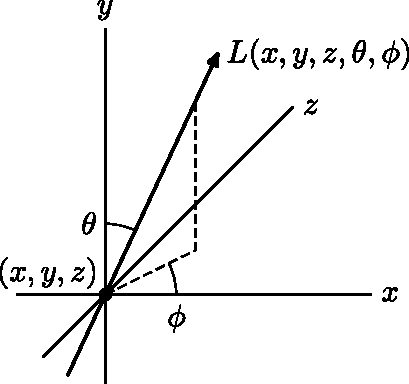
\includegraphics[width=.4\textwidth]{obrazky-figures/plenoptic-function.pdf}
	\caption{Ilustrace plenoptické funkce. Pro zjednodušení není brán v úvahu čas a vlnová délka světla.}
	\label{plenoptic-function}
\end{figure}

Formálně lze plenoptickou funkci definovat jako $P(x, y, z, \theta, \phi, \lambda, t)$, kde
\begin{itemize}
  \item $x, y, z, t$ jsou časoprostorové souřadnice,
  \item $\theta, \phi$ definují prostorový úhel světelného paprsku,
  \item $\lambda$ je vlnová délka světelného paprsku.
\end{itemize}

Jelikož je funkce definovaná v každém bodě v časoprostoru, lze pomocí ní vyjádřit každou scénu, každou fotografii a každý film.
Všechno, co kdy bylo, je a bude viděno.
Naneštěstí toto není v reálném světě možné, proto slouží plenoptická funkce pouze jako idealizovaný koncept.

Tento koncept má však spoustu reálných uplatnění. Příkladem může být třeba první monochromatická fotografie zachycená pomocí dírkové komory.
Tuto fotografii lze definovat jako plenoptickou funkci integrovanou přes viditelné spektrum světla se souřadnicemi ve středu otvoru dírkové komory v čase pořízení a v určitém rozsahu úhlů $\theta, \phi$.
Tyto úhly si lze volně představit jako vertikální a horizontální souřadnice na výsledné fotografii.
Fotografie ve stupních šedi je proto dvourozměrná funkce $F(\theta, \phi)$.

Podobně lze definovat barevnou fotografii jako trojrozměrnou funkci $F(\theta, \phi, \lambda)$, kde oproti monochromatické fotografii není přes vlnovou délku integrováno.
$\lambda$ se tak stává třetím parametrem.
Pokud je k funkci dvourozměrné barevné fotografie přidán parametr $t$, který reprezentuje čas, vznikne čtyřrozměrná funkce $F(\theta, \phi, \lambda, t)$, která reprezentuje video.
Dalším příkladem může být funkce $F(x, y, z, \theta, \phi, \lambda)$ která není parametrizována časem, ale prostorovými souřadnicemi $x, y, z$.
Tato funkce je kompletní holografickou reprezentací zachycené scény v daném čase.

Důležitost plenoptické funkce proto spočívá v tom, že pomocí jejich řezů lze definovat různé reprezentace zachycené scény.
Jedním z těchto řezů je také 4D světelné pole, kterému se věnuje následující podkapitola.

\section{4D světelné pole}
\label{4D-light-field}
Čtyřrozměrné světelné pole je jedním z mnoha řezů plneoptické funkce.
Tento řez je definován funkcí $F(x, y, \theta, \phi, \lambda)$.
Pozorný čtenář si všimne, že funkce má o jeden rozměr víc, než deklaruje její název.
Jde o vlnovou délku $\lambda$.
Ačkoli se v praxi s barevnými kanály pracuje, v literatuře se pro zjednodušení zanedbává, protože se světelným polem přímo nesouvisí.
Toto zjednodušení je zavedeno i ve zbytku této kapitoly, světelné pole je tedy definováno funkcí $F(x, y, \theta, \phi)$.

Vychází se z předpokladu, že světelné paprsky putující prostorem obvykle nemění svůj směr.
Tím pádem vzniká v plenoptické funkci redundance, protože jeden světelný paprsek se promítne do všech bodů v prostoru $x, y, z$, skrz které tento paprsek prochází.
Tato redundance je podrobněji vykreslena na obrázku \ref{redundance}.
Světelné pole oproti tomu zachycuje paprsek právě jednou, a to v bodě, kde se tento paprsek setkává s rovinou $x, y$.
To demonstruje obrázek \ref{neredundance}.

Čtyřrozmerné světelné pole tedy obsahuje kompletní reprezentaci statické scény pozorované z jedné roviny v prostoru a slouží jako formální aparát pro plenoptické fotografie.

\section{Zachycení plenoptické fotografie}
\label{light-field-capture}
\begin{figure}[h]
  \centering
  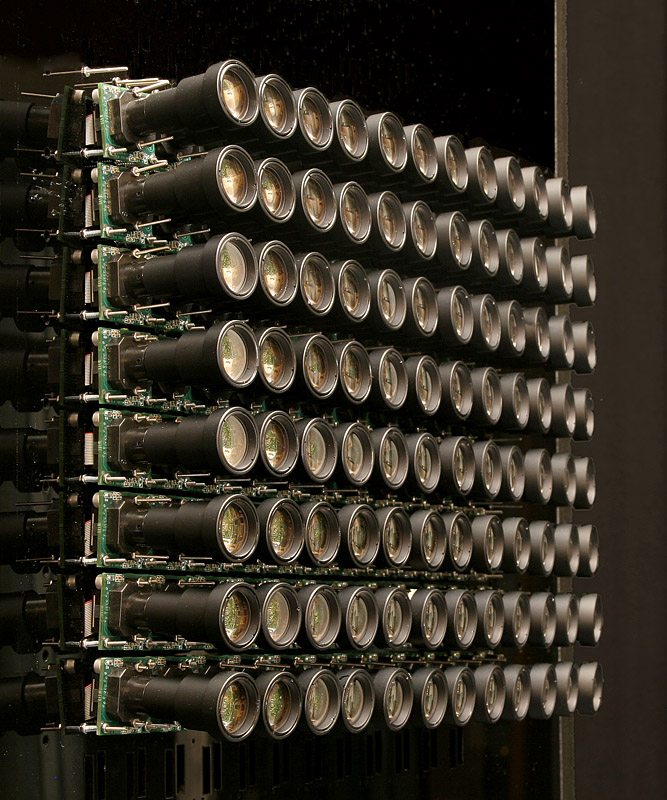
\includegraphics[width=.4\textwidth]{obrazky-figures/stanford-array.jpg}
	\caption{Pole fotoaparátů sestrojené na univerzitě Stanford \cite{stanford}.}
	\label{stanfordArray}
\end{figure}

Nejjednoduším způsobem zachycení plenoptické fotografie je pole klasických dvourozměrných fotoaparátů, které jsou rovnoměrně rozloženy v rovině.
Na obrázku \ref{stanfordArray} je možné vidět, jak takové pole vypadá.
Scéna je zachycena všemi fotoaparáty ve stejném čase.
Fotografie zachycená jedním fotoaparátem reprezentuje jeden snímek plenoptické fotografie.
Index pohledu je dán indexem fotoaparátu, který tento pohled vyfotografoval.
Z pole snímků lze vypočítat hloubková data.

Komplikovanější variantou může být specializovaný plenoptický fotoaparát.
Oproti klasickému fotoaparátu se liší tím, že má před světlocitlivým senzorem pole mikročoček.
Paprsek světla přicházející do fotoaparátu je nejprve hlavní čočkou soustředěn do pole mikročoek, které jej podle úhlu dopadu rozptýlí na světlocitlivý senzor.
Tento princip je vyobrazen na obrázku \ref{plenoPrincip}.
Každá mikročočka zachytává jeden pixel scény z více pohledů.
Této jednotce se říká makropixel.

\begin{figure}
	\centering
		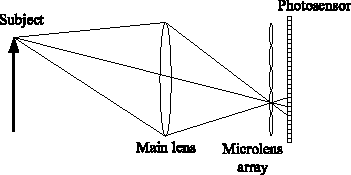
\includegraphics[width=.4\textwidth]{obrazky-figures/pleno-cam.pdf}
		\caption{Princip plenoptického fotoaparátu. Paprsky směřující do fotoaparátu jsou před zachycením na světlocitlivý senzor rozptýleny polem mikročoček.}
		\label{plenoPrincip}
\end{figure}

\section{Formáty pro uložení plenoptických dat}
\label{light-field-formats}
Plenoptická data můžou mít různé formáty a každý formát je vhodný pro jiné využití.
Na jednu stranu je potřeba s těmito daty pracovat rychle a efektivně, na stranu druhou se musí řešit paměťové nároky na uložení těchto dat a s tím související komprese.

Při práci s plenoptickým fotoaparátem se lze nejčastěji setkat s daty v lenslet\footnote{Lenslet -- mikročočka, která je prvkem pole mikročoček \cite{lenslet}.} formátu. Jde o surová data, která jsou zachycena světlocitlivým senzorem v plenoptickém fotoaparátu.
Tato data reflektují rozložení mikročoček ve fotoaparátu.
Pro jejich snažší zpracování jsou k samotné bitmapě přiložena metadata o konstrukci fotoaparátu, který tato data zachytil.
Mimo metadata, která ukládá klasický fotoaparát, se zde zaznamenává zejména informace o velikosti a rozložení mikročoček.

Další alternativou, jak ukládat plenoptické fotografie, je dvourozměrné pole pohledů na tutéž scénu, kde každý pohled reprezentuje snímek scény pod jiným úhlem pozorování.
Tento formát je obvykle výstupem zachycení plenoptické fotografie pomocí dvourozměrného pole fotoaparátů.
Jako metadata jsou v tomto případě uloženy koordináty jednotlivých pohledů, a to buď ve formě vertikálního a horizontálního indexu, nebo lépe také pomocí jednotek reálného světa.
Druhá varianta umožňuje určit měřítko zachycené scény a tím i rozměry objektů, které se ve scéně nacházejí.

Tento formát je vhodný zejména pro kompresi založenou na transformaci a kvantizaci.
Příznivým faktorem pro tuto třídu kompresních algoritmů je silná korelace mezi jednotlivými sousedícími pohledy.
Proto se plenoptické fotografie zachycené plenoptickým fotoaparátem do tohoto formátu často převádí.

Plenoptická data je také možné ukládat jako point cloud\footnote{Point cloud -- množina bodů v prostoru.}.
Tento formát již nezaznamenává paprsky světla zachycené na senzor, nýbrž rekonstruovanou trojrozměrnou scénu, kterou toto světlo reprezentuje.
Point cloud, případně polygonová síť z point cloudu vytvořená, je vhodná pro vykreslení běžnými renderovacími algoritmy.



\chapter{Principy ztrátové komprese využitelné pro plenoptická data}
\label{kompres-teo}
Ztrátová komprese je komprese, při které dochází k nezvratné ztrátě informací, rekonstruovaná data tedy pouze aproximují data původní.
Výhodou dobře implementované ztrátové komprese oproti bezeztrátové kompresi je signifikantní redukce velikosti oproti zanedbatelné degradaci dat.
Díky nedokonalosti lidských smyslů je ztrátová komprese hojně využívaná v oblasti obrazových a zvukových signálů.
U ztrátové komprese je snaha redukovat data, která mají nejmenší význam.

\section{Komprese obrazu}
Nejrozšířenějším standardem pro ztrátovou kompresi se obrazu stal formát JPEG z roku 1992.
Tento formát je založený na diskrétní cosinově transformaci a následné kvantizaci výsledných koeficientů podle citlivosti lidského oka na jednotlivé frekvence v obrazu.

\section{Kompresní řetězec JPEG}
\label{jpeg}

\subsubsection*{Transformace barevného prostoru}

RGB obrázek je vhodné před samotnou transformací převést do vhodného barevného modelu.
K tomuto se vybízí využít model YC\textsubscript{b}C\textsubscript{r}, který barevná data dělí na luminanci Y (jas) a složky chrominance C\textsubscript{b}C\textsubscript{r} (barvy).
Jelikož je lidské oko citvlivé více na jas než na barvu, je možné chromatické složky komprimovat více drasticky bez viditelné ztráty kvality.
Po převodu do vhodného barevného modelu je každý kanál komprimován zvlášť.

\subsubsection*{Dělení do bloků}

Data jednoho komprimovaného kanálu jsou převedeny do bloků velikosti $8\times8$, které jsou následně komprimovány individuálně.
U obrázků, jejichž rozměr není násobkem osmi, vzniká problém krajních bloků.
Obrázek se v tomto případě obvykle rozšíří na násobek osmičky, přičemž existuje několik alternativ, jak vyplnit nově vytvořené krajní pixely.
Nejjednodušší je vyplnit prázdné místo nějakou jednotnou barvou.
Nevýhodou tohoto přístupu je vysoká frekvence, která vzniká skokovým přechodem mezi obrázkem a barvou.
Tento problém dokáže částečně řešit přístup, kdy se redundantní pixely doplní hodnotou krajních pixelů originálního obrázku.
Alernativou může být také zrcadlení původního obrázku nebo jeho opakování (svinutí obrázku do pomyslného torusu).

\subsubsection*{Diskrétní cosinova transformace}

Na každý blok se dále aplikuje diskrétní cosinova transformace.
DCT rozloží blok na DC koeficient -- vlevo nahoře -- reprezentující pouze průměrnou barvu bloku, a AC koeficienty -- všechny ostatní -- reprezentující jednotlivé frekvence.
Jde o transformaci podobnou diskrétní Fourierově transformaci, která produkuje pouze reálné koeficienty.
Diskrétní cosinova transformace je využívána také z důvodu koncentrace nejvíce energie na nejnižších frekvencích, což je z hlediska ztrátové komprese výhodné.

\subsubsection*{Kvantizace}

Na transformované bloky se aplikuje kvantizace.
Kvantizace je jádro ztrátové komprese, v tomto kroku jsou totiž aplikovány ztráty.
Ke kvantizaci se využívá kvantizační matice.
Tato matice byla vytvořena na základě experimentů zkoumajících vlastnosti lidského oka.
Je navržena tak, aby redukovala frekvence, na které je lidské oko nejméně citlivé.
Kvantizace probíhá podělením DCT koeficientů hodnotou v kvantizační matici a následným zaokrouhlením.
Kvantizace má za následek, že většina výsledných koeficientů má hodnotu nula.
Toho je využito zejména v bezeztrátové kompresi, která následuje.

\subsubsection*{Entropické kódování}

Dále je potřeba blok převést do 1D, avšak tak, aby byly kvantizované koeficienty v nejlepším případě seřazeny od největšiho po nejmenší.
K tomu se využívá průchod způsobem cik-cak.
Tento průchod zajišťuje, že DC koeficient bude na jedné straně a AC koeficient s největšimi vertikálními a horizontálnímí frekvencemi bude na straně druhé.

Na DC koeficienty je aplikováno kódování, kdy je od každého DC koeficientu odečten DC koeficient předchozího bloku.
Tyto rozdíly se uloží namísto původních DC koeficientů.

AC koeficienty jsou zakódovány pomocí RLE\footnote{RLE -- Run-length encoding.}.
RLE je provedeno tak, že každý nenulový koeficient v bloku je převeden na dvojici (ZEROES, AMPLITUDE), kde ZEROES je počet nul, které koeficientu předcházely, a AMPLITUDE je samotná hodnota koeficientu.

Toto kódování zahrnuje dvě speciální dvojice.
Tou první je dvojice (0, 0), takzvaný EOB\footnote{EOB -- End-of-block.} -- symbol sloužící jako ukončující značka daného bloku reprezentující zbytek nul na konci.
Kvůli tomu je pro kompresi výhodné řadit koeficienty tak, aby na konci bylo velké množství nul.
Pokud nastane situace, kde je před kódovaným nenulovým koeficientem více než 15 nul, je nutné zavést opatření, která zajistí, že hodnotu počtu nul bude možné uložit do 4 bitů.
Tímto opatřením je dvojice (15, 0), která reprezentuje šestnáct nulových koeficientů za sebou, resp. patnáct předcházejících nul + koeficient s nulovou hodnotou.
Pokud se tedy na vstupu objeví napříkad sedmnáct nul a dvojka, budou výstupem dvojice (15, 0) a (1, 2).

Pro efektivní entropické kódování by bylo vhodné, kdyby měl kódovaný symbol nějakou vhodnou délku.
V předchozím odstavci bylo zmíněno, že ZEROES je hodnota, která se vejde na čtyři bity.
Oproti tomu maximální velikost AMPLITUDE závisí na použité metodě DCT a v obvyklých případech dosahuje až 11 bitů.
Proto metoda JPEG nekóduje dvojice (ZEROES, AMPLITUDE), ale (ZEROES, SIZE), kde SIZE je index nejvyššího jedničkového bitu v absolutní hodnotě kódované amplitudy, ke kterému je přičtena jednička.
Amplituda s hodnotou nula neobsahuje žádný jedničkový bit, hodnota SIZE je v tomto případě 0.
Položka SIZE je bezznaménková a může dosahovat maximální hodnoty 11, k uložení této hodnoty proto vystačí čtyři bity.
Jelikož je každá z těchto hodnot kódovaná na čtyřech bitech, je možné obě tyto hodnoty uložit do jednoto bytu.
Tento byte je symbolem, který je dále entropicky kódován.

Symboly se kódují buď pomocí Huffmanova kódování, nebo pomocí aritmetického kódování.
Huffmanovo kódování je rozšířené pro svoji menší výpočetní náročnost.
K zakódování lze využít již existující huffmanovu tabulku.
Předpočítaná tabulka výrazně šetří čas, ovšem za cenu suboptimální komprese.
Oproti tomu lze huffmanovu tabulku vypočítat speciálně pro pravděpodobnostní rozložení dané kódovaným obrázkem.
Za cenu větší výpočetní náročnosti je proto možné vygenerovat optimální huffmanovu tabulku pro optimální krok bezeztrátové komprese.

V metodě JPEG se obvykle používají zvlášť huffmanovy tabulky pro AC a DC koeficienty a zvlášť také pro luminanci a chrominanci.
Celkem tedy $(AC, DC)\times(luma, chroma)$ čtyři huffmanovy tabulky.
Tyto tabulky jsou uloženy ve výsledném souboru.
Komprese huffmanovy tabulky je možná při použití kanonického huffmanova kódování.

Aritmetické kódování dosahuje lepšího kompresního poměru za cenu větší výpočetní náročnosti při kódování a dekódování.
Proto tato není tak často využívaná v praxi.

Samotná amplituda není entropicky kódovaná, ale ukládá se jen na zakódovaný potřebný počet bitů.
Záporné hodnoty amplitudy se ukládají v jedničkovém doplňku.

\chapter{Implementace kodeku plenoptických fotografií}
\label{lfif-impl}

\chapter{Závěr}
%\label{zaver}




%===============================================================================
